\documentclass[conference]{IEEEtran}

\usepackage{amsmath,amssymb}
\usepackage{graphicx}
\usepackage{booktabs}
\usepackage{url}
\usepackage[hidelinks]{hyperref}
\usepackage{xcolor}
\graphicspath{{../figures/}}
\hypersetup{
  pdftitle={Reliability-Focused Machine-Failure Prediction Under Imbalanced and Degraded Sensor Data},
  pdfauthor={MAA AACAAS MUHAMATH},
  pdfsubject={Reliability evaluation of machine-failure prediction on AI4I 2020},
  pdfkeywords={predictive maintenance, class imbalance, sensor corruption, missing data, Random Forest}
}

\title{Reliability-Focused Machine-Failure Prediction Under Imbalanced and Degraded Sensor Data}

\author{\IEEEauthorblockN{MAA AACAAS MUHAMATH}
\IEEEauthorblockA{Department of Electrical Engineering\\
University of Moratuwa\\Moratuwa, Sri Lanka}}

\begin{document}
\maketitle

\begin{abstract}
Machine-failure classifiers are often assessed on clean data even though deployment may involve rare failures, noisy measurements, missing sensor values, and limited labelled data. This study evaluates an unweighted 300-tree Random Forest on the synthetic AI4I 2020 benchmark using six predictors, a stratified 70/15/15 split, and a validation-selected threshold of 0.20. On the untouched test set, the classifier achieved 0.5676 precision, 0.8235 recall, 0.6720 F1, and 0.7803 Average Precision (AP), detecting 42 of 51 failures. A Wilson interval places recall at 0.6975--0.9043; stratified bootstrap intervals were 0.4824--0.6667 for precision, 0.5891--0.7563 for F1, and 0.6816--0.8717 for AP. Repeated robustness experiments evaluated nonzero corruption conditions over 30 seeds and reduced-data conditions over 20 stratified seeds. At 30\% Gaussian noise, mean recall was 0.6791 and mean AP was 0.4596. At 30\% MCAR-style synthetic missingness, mean recall was 0.5229 while mean accuracy remained 0.9703. With 20\% of labelled training data, mean recall was 0.6510 and mean AP was 0.5854. These results support a narrow conclusion: strong clean-data accuracy can coexist with materially weaker minority-class detection under degraded sensing. The evidence characterizes one model on one synthetic benchmark and does not establish field generalization.
\end{abstract}

\begin{IEEEkeywords}
predictive maintenance, machine failure, class imbalance, sensor corruption, missing data, Random Forest, uncertainty, explainability
\end{IEEEkeywords}

\section{Introduction}
Condition-based and predictive maintenance use monitored operating data to support diagnostics, prognostics, and maintenance decisions \cite{jardine2006review}. Machine learning has consequently become common in predictive-maintenance research \cite{carvalho2019review,zonta2020review,susto2015pdm}. Yet a model evaluated only on clean observations can appear dependable while remaining sensitive to sensor degradation. The issue is amplified when failures are rare: a system may correctly classify most healthy machines and retain high accuracy while missing a large fraction of failures.

This paper presents a reliability-focused evaluation on the AI4I 2020 benchmark. AI4I is useful and openly available, but it is synthetic rather than a record of a deployed industrial fleet \cite{uci_ai4i,matzka2020xai}. Accordingly, the objective is not a claim of industrial readiness or a new learning algorithm, but a transparent robustness characterization of a fixed classifier and operating threshold.

The study addresses five research questions:
\begin{enumerate}
\item[RQ1:] How effectively does the selected system detect the minority failure class under its validation-selected operating policy?
\item[RQ2:] How does performance change as numerical sensor measurements receive increasing Gaussian noise?
\item[RQ3:] How does increasing missing sensor information affect failure detection?
\item[RQ4:] How sensitive is performance to reductions in labelled training data?
\item[RQ5:] Which features are most associated with predictions, especially correctly detected and missed failures?
\end{enumerate}

The contribution is an auditable reliability evaluation comprising: (i) clean-data performance at a validation-selected operating threshold; (ii) explicit uncertainty for the small failure test sample; (iii) repeated-seed noise, missingness, and label-scarcity experiments; and (iv) threshold, calibration, explainability, and post-hoc failure-mode diagnostics.

\section{Related Work}
Predictive maintenance combines sensing, data processing, and decisions about equipment intervention \cite{jardine2006review}. Reviews identify broad adoption of statistical and machine-learning approaches but also emphasize heterogeneous assets, data availability, and evaluation practices \cite{carvalho2019review,zonta2020review,dalzochio2020status}. Susto \emph{et al.} showed how multiple classifiers and operating horizons can support maintenance trade-offs \cite{susto2015pdm}. IoT-enabled maintenance further exposes models to communication, integration, and data-quality challenges \cite{compare2020iot}.

AI4I was introduced as a realistic but synthetic predictive-maintenance dataset with an explainability demonstration \cite{matzka2020xai}. Its accessibility supports reproducible comparison, but synthetic generation and a single fixed dataset limit external validity. This work therefore treats AI4I as a controlled benchmark rather than a substitute for prospective industrial validation.

Imbalanced learning requires attention beyond accuracy \cite{he2009imbalance}. Sampling methods such as SMOTE address training imbalance \cite{chawla2002smote}; this study instead evaluates an unweighted Random Forest under a fixed operating policy. Precision--recall evaluation is informative when the positive class is rare \cite{saito2015pr,davis2006pr}. AP is reported here because the implementation uses \texttt{average\_precision\_score}; it is not labelled generically as PR-AUC.

Decision thresholds convert ranking scores into operational actions. Threshold selection changes the precision--recall trade-off and must be separated from final test evaluation \cite{lipton2014threshold}. The present threshold was fixed on validation data before the test set was evaluated. Calibration is related but distinct: it asks whether scores correspond to observed frequencies \cite{brier1950score,niculescu2005probabilities,guo2017calibration}.

Missingness mechanisms matter. Rubin's framework distinguishes missingness assumptions \cite{rubin1976missing}; broader treatments warn that simple synthetic removal does not represent all real missing-data processes \cite{little2019missing,vanbuuren2018imputation}. The experiment here is explicitly characterized as MCAR-style synthetic missingness. It does not model correlated dropout, drift, or failure-dependent sensor loss.

Uncertainty is especially important with few positive examples. Wilson score intervals avoid some defects of naive Wald intervals for binomial proportions \cite{wilson1927interval}; bootstrap resampling provides a practical way to characterize sampling variability for nonlinear metrics \cite{efron1993bootstrap}. Explainability methods describe model associations, not physical causes. SHAP provides additive feature attributions \cite{lundberg2017shap}; permutation methods assess predictive reliance under feature perturbation \cite{fisher2019reliance}; local explanations require equally careful interpretation \cite{ribeiro2016lime}.

\section{Dataset and Problem Formulation}
The UCI AI4I 2020 dataset contains 10,000 records, of which 339 (3.39\%) have \texttt{Machine failure}=1 \cite{uci_ai4i}. The six predictors are machine type, air temperature, process temperature, rotational speed, torque, and tool wear. The component indicators TWF, HDF, PWF, OSF, and RNF are excluded from model inputs because they describe failure mechanisms and would leak target information. They are used only for post-hoc diagnostics.

The stratified 70/15/15 split is shown in Table~\ref{tab:distribution}. The 1,500-record test set contains only 51 failures. Let $p_i$ denote the model score and $t=0.20$ the fixed operating threshold. Predictions are $\hat y_i=\mathbb{1}[p_i\geq t]$.

\begin{table}[t]
\caption{Stratified Data Split}
\label{tab:distribution}
\centering
\begin{tabular}{lrrr}
\toprule
Partition & Records & Failures & Failure rate (\%)\\
\midrule
Training & 7000 & 237 & 3.39\\
Validation & 1500 & 51 & 3.40\\
Test & 1500 & 51 & 3.40\\
\bottomrule
\end{tabular}

\end{table}

\section{Methodology}
\subsection{Core Prediction Protocol}
Preprocessing was fitted on training data only. Numerical variables were median-imputed without scaling for the tree model; machine type was one-hot encoded. Baselines comprised a majority Dummy Classifier, unweighted Logistic Regression, and an unweighted Random Forest \cite{breiman2001rf,pedregosa2011sklearn}. The selected forest used 300 trees, \texttt{random\_state=42}, and no class weighting.

Validation analysis evaluated thresholds from 0.05 to 0.50. Threshold 0.20 was selected as a safety-oriented point because validation recall was at least 0.80 with a manageable false-positive count. It was not the validation F1 optimum: threshold 0.40 had the highest F1 on that grid. The selected 0.20 policy was then fixed for the clean test, corruption, reduced-data, and explainability experiments. The test set was not used for threshold optimization.

Initial robustness checks used single seeded realizations. Gaussian noise at 0, 5, 10, 20, and 30\% was scaled by each feature's standard deviation computed on the test data. Missing numerical cells were independently masked using a fixed seed and filled with training medians. Reduced-data checks retrained on one stratified subset at each of 20, 40, 60, 80, and 100\% of training data.

\subsection{Repeated Robustness Evaluation}
Repeated experiments used the same split, six features, forest configuration, and threshold. For numerical feature $j$, Gaussian corruption at severity $s$ was defined as
\begin{equation}
x'_{ij}=x_{ij}+\epsilon_{ij},\qquad
\epsilon_{ij}\sim\mathcal{N}\!\left(0,\left(s\sigma^{\mathrm{train}}_j\right)^2\right),
\label{eq:noise}
\end{equation}
where $\sigma^{\mathrm{train}}_j$ is the standard deviation estimated from the training partition and $s\in\{0,0.05,0.10,0.20,0.30\}$. The categorical machine-type feature was not corrupted. Each nonzero severity was repeated across 30 seeds. Missingness was produced by independent Bernoulli masks over test-set numerical cells, repeated across the same 30 seeds, and imputed with training medians. This is an MCAR-style stress test, not a model of all industrial missingness.

For label scarcity, 20 stratified subsamples were drawn at each fraction below 100\%; a fresh preprocessor and Random Forest were fitted for every replicate. The full-data point is deterministic and therefore reported once. Replicate summaries report the mean, standard deviation, and normal-approximation 95\% interval for the mean. These intervals quantify Monte Carlo variation across synthetic corruptions or subsets, not variation across independent industrial datasets.

Clean-test recall uses a Wilson interval because it is a binomial sensitivity estimate over 51 failures. Precision, F1, and AP use a 5,000-replicate stratified percentile bootstrap that separately resamples positive and negative test records. Calibration is summarized by the Brier score and a quantile-binned reliability diagram. No calibrated classifier replaces the evaluated model or threshold.

Permutation importance measures the decrease in test AP over 30 shuffles. SHAP values are aggregated by confusion group (TP, FN, FP, TN). Failure modes are examined only after prediction. Because mechanisms can overlap and groups are small, their recalls are descriptive.

\section{Results}
\subsection{Baseline Comparison and Threshold}
Table~\ref{tab:baselines} reports validation outputs at the default 0.50 threshold. The Random Forest provided the highest F1 and AP. Current-environment reproduction matched the recorded Dummy and Logistic Regression values and Random Forest AP to four decimals, but produced one additional Random Forest false positive (six rather than five), changing precision from 0.8387 to 0.8125. This minor library-version sensitivity does not affect the independently reproduced selected-threshold test result.

\begin{table}[t]
\caption{Validation Baselines at Threshold 0.50}
\label{tab:baselines}
\centering
\begin{tabular}{lrrrr}
\toprule
Model & Precision & Recall & F1 & AP\\
\midrule
Dummy Classifier & 0.0000 & 0.0000 & 0.0000 & 0.0340\\
Logistic Regression & 0.6364 & 0.1373 & 0.2258 & 0.3844\\
Random Forest & 0.8387 & 0.5098 & 0.6341 & 0.7349\\
\bottomrule
\end{tabular}

\end{table}

Figure~\ref{fig:threshold} shows the validation threshold trade-off. The formal supplementary rule ``maximize precision subject to recall $\geq0.80$'' also selects 0.20 on the evaluated grid, providing a transparent consistency check for the selected operating point.

\begin{figure}[t]
\centering
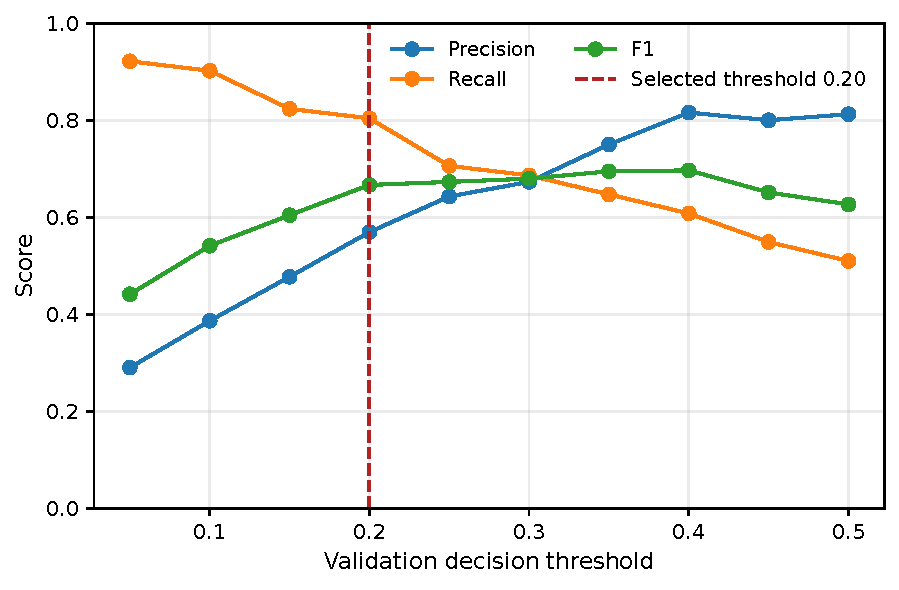
\includegraphics[width=\columnwidth]{validation_threshold_tradeoff.pdf}
\caption{Validation precision, recall, and F1 across the evaluated threshold grid. Threshold 0.20 was selected before final test evaluation.}
\label{fig:threshold}
\end{figure}

\subsection{Clean Test Performance and Uncertainty}
The clean result reproduced exactly: TN=1417, FP=32, FN=9, TP=42; accuracy=0.9727, precision=0.5676, recall=0.8235, F1=0.6720, and AP=0.7803. Table~\ref{tab:clean} shows uncertainty. The recall interval is wide (0.6975--0.9043), reflecting only 51 test failures. Thus 0.8235 should not be read as a precise population sensitivity.

\begin{table}[t]
\caption{Clean Test Estimates and 95\% Intervals}
\label{tab:clean}
\centering
\begin{tabular}{lrrr}
\toprule
Metric & Estimate & 95\% lower & 95\% upper\\
\midrule
Precision & 0.5676 & 0.4824 & 0.6667\\
Recall & 0.8235 & 0.6975 & 0.9043\\
F1 & 0.6720 & 0.5891 & 0.7563\\
Average Precision & 0.7803 & 0.6816 & 0.8717\\
\bottomrule
\end{tabular}

\end{table}

The precision--recall curve is shown in Fig.~\ref{fig:pr}. AP substantially exceeds the test prevalence baseline of 0.034, but this held-out ranking result remains dataset-specific.

\begin{figure}[t]
\centering
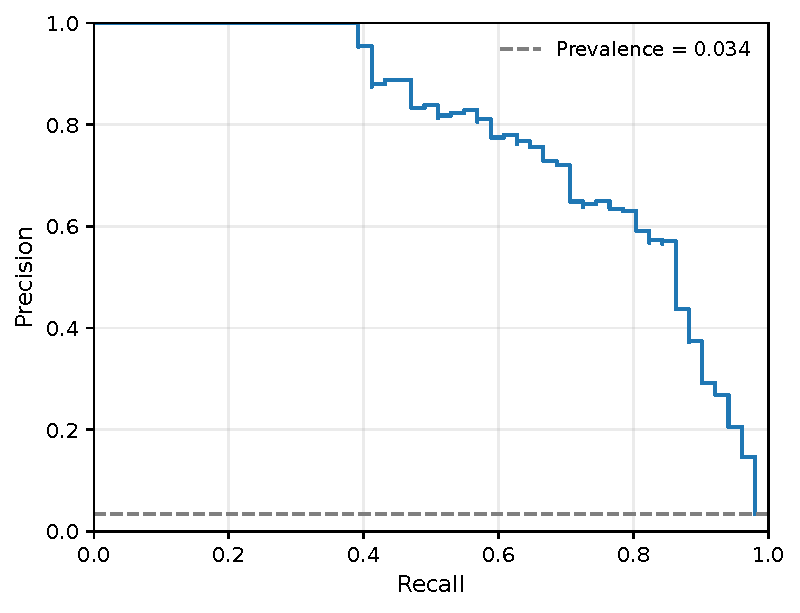
\includegraphics[width=0.92\columnwidth]{test_precision_recall_curve.pdf}
\caption{Held-out test precision--recall curve for the Random Forest; AP=0.7803.}
\label{fig:pr}
\end{figure}

\subsection{Repeated Robustness Results}
Table~\ref{tab:robust} summarizes representative severe conditions. Under 30\% training-scaled Gaussian noise, mean recall was 0.6791 (SD 0.0493) and mean AP was 0.4596 (SD 0.0540). At 30\% MCAR-style missingness, mean recall was 0.5229 (SD 0.0528) and mean AP was 0.4918 (SD 0.0596), while mean accuracy remained 0.9703. The stable accuracy therefore masks a large reduction in failure detection.

\begin{table*}[t]
\caption{Performance Under Representative Robustness Conditions}
\label{tab:robust}
\centering
\begin{tabular}{lrrrr}
\toprule
Condition & Precision & Recall & F1 & AP\\
\midrule
Clean test & 0.5676 & 0.8235 & 0.6720 & 0.7803\\
30\% Gaussian noise & 0.3129 & 0.6791 & 0.4282 & 0.4596\\
30\% MCAR-style missingness & 0.5709 & 0.5229 & 0.5447 & 0.4918\\
20\% labelled training data & 0.4679 & 0.6510 & 0.5420 & 0.5854\\
\bottomrule
\end{tabular}

\end{table*}

Figures~\ref{fig:noise} and \ref{fig:missing} show mean recall and AP with intervals for the mean. The initial single-seed 30\% results are reported separately: noise recall 0.6667 and AP 0.5417; missingness recall 0.5098 and AP 0.5432. The repeated evaluation confirms the direction of degradation while showing seed-dependent variability and, for noise AP, a lower repeated mean under the leakage-safe scaling protocol.

\begin{figure}[t]
\centering
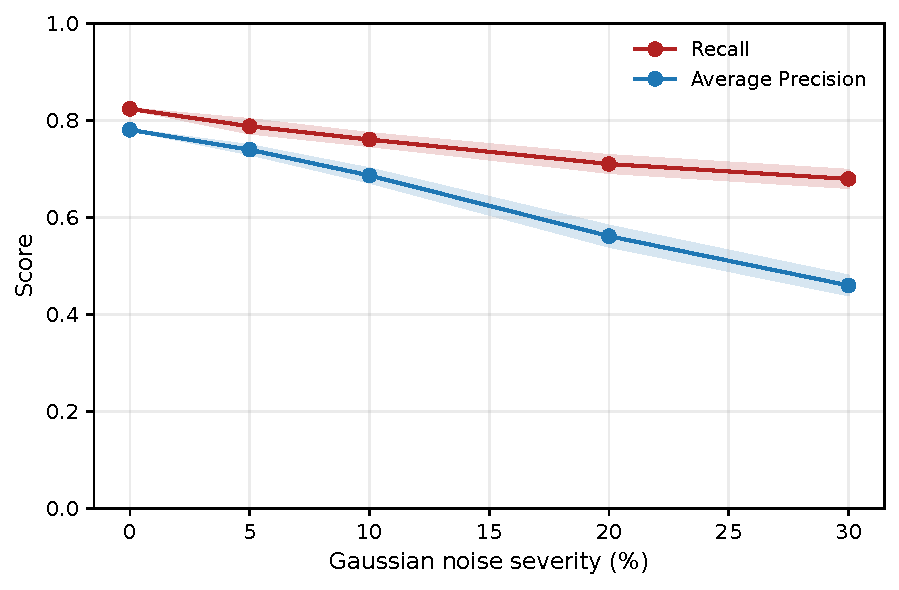
\includegraphics[width=\columnwidth]{repeated_sensor_noise.pdf}
\caption{Repeated Gaussian-noise evaluation. Bands are 95\% intervals for the mean over 30 seeds at nonzero levels.}
\label{fig:noise}
\end{figure}

\begin{figure}[t]
\centering
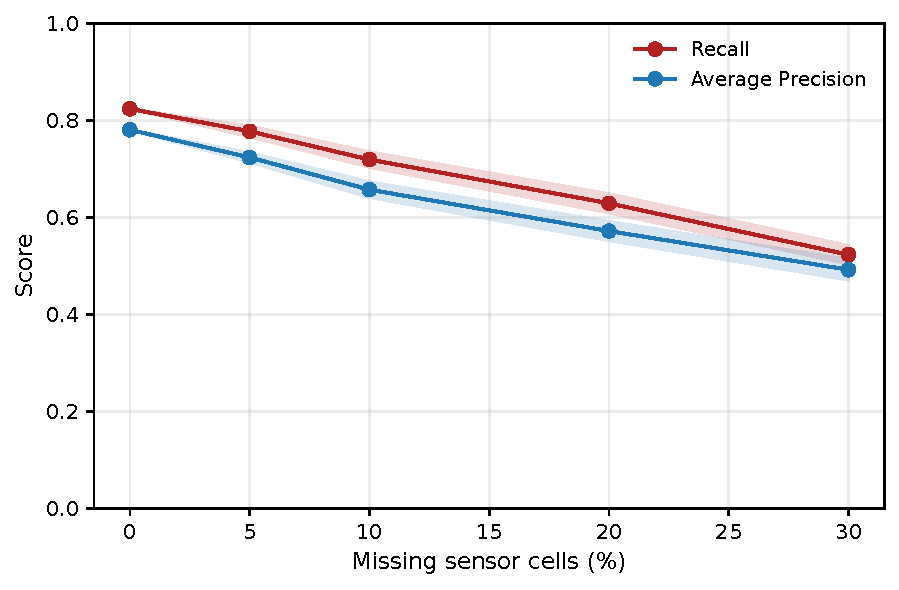
\includegraphics[width=\columnwidth]{repeated_missing_data.pdf}
\caption{Repeated MCAR-style missingness evaluation with training-median imputation.}
\label{fig:missing}
\end{figure}

With 20\% of labelled training data, mean recall was 0.6510 (SD 0.0799), mean F1 was 0.5420 (SD 0.0397), and mean AP was 0.5854 (SD 0.0584). Mean AP rose monotonically across fractions to the deterministic full-data value 0.7803. The initial 20\% single subset achieved recall 0.6667 and AP 0.6546; the repeated analysis shows that one subset overstated the average AP observed across 20 subsets.

\begin{figure}[t]
\centering
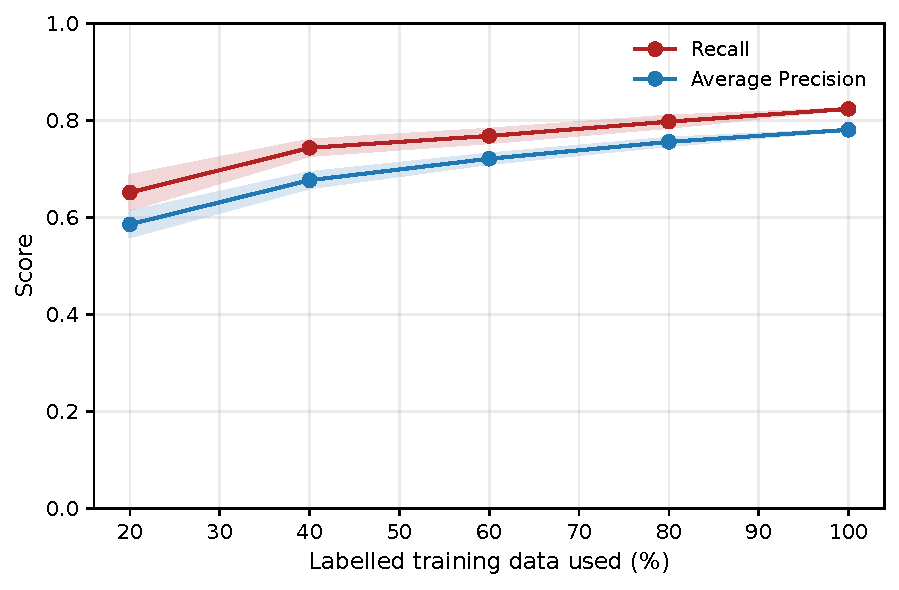
\includegraphics[width=\columnwidth]{repeated_label_scarcity.pdf}
\caption{Repeated stratified labelled-data-scarcity evaluation. Non-full fractions use 20 seeds.}
\label{fig:scarcity}
\end{figure}

\subsection{Calibration}
The unmodified Random Forest had a Brier score of 0.01542 on the test set. Figure~\ref{fig:calibration} suggests approximate agreement in the highest quantile bin (mean score 0.278, observed frequency 0.307), but the small positive count and coarse quantile bins preclude strong calibration claims. This supplementary check does not alter the classifier or operating threshold.

\begin{figure}[t]
\centering
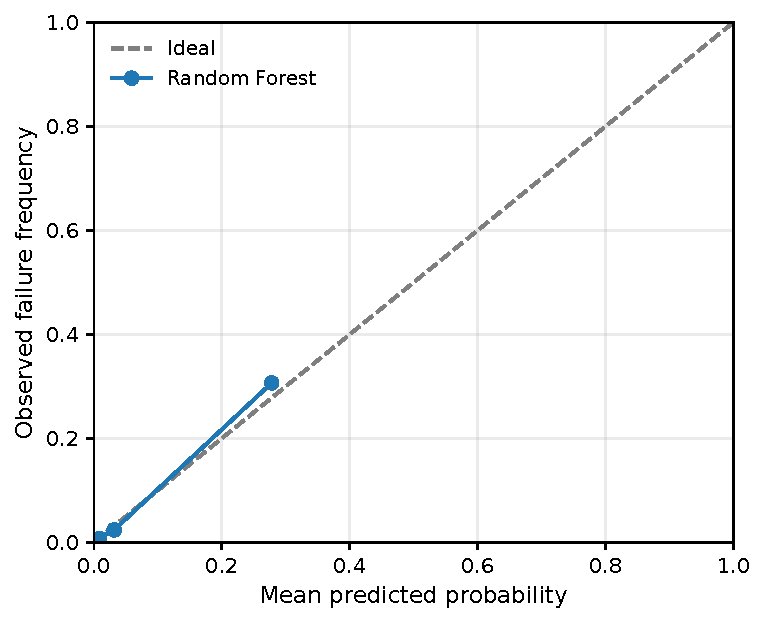
\includegraphics[width=0.92\columnwidth]{reliability_diagram.pdf}
\caption{Supplementary reliability diagram for Random Forest scores.}
\label{fig:calibration}
\end{figure}

\section{Explainability and Error Analysis}
Impurity-based importance ranked torque first (0.3245), followed by rotational speed (0.2372) and tool wear (0.1671). Permutation importance using AP agreed on torque as the strongest feature (mean AP decrease 0.5107), followed by rotational speed (0.3372), air temperature (0.2999), tool wear (0.2871), and process temperature (0.1603). Machine-type indicators were near zero. Correlated features can share or distort permutation importance; neither measure implies causation.

A SHAP example for a correctly detected failure ($p=0.94$) was dominated by rotational speed (+0.5036) and torque (+0.3625). A selected false negative ($p=0.1367$) had weaker and conflicting contributions: rotational speed +0.0910, air temperature +0.0906, process temperature -0.0684, tool wear -0.0206, and torque +0.0143. Confusion-group analysis likewise found mean absolute torque SHAP of 0.2123 among 42 TPs but only 0.0237 among 9 FNs; mean absolute rotational-speed SHAP was 0.1365 for TPs and 0.0457 for FNs. These are model attributions associated with predictions, not causal mechanisms.

Post-hoc failure-mode results are shown in Table~\ref{tab:modes}. HDF, PWF, and OSF cases were often detected, whereas only 2 of 8 TWF cases and neither of 2 RNF cases were detected. Mechanisms overlap, denominators are extremely small, and no inferential conclusion should be drawn.

\begin{table}[t]
\caption{Post-hoc Failure-Mode Diagnostics}
\label{tab:modes}
\centering
\begin{tabular}{lrrrr}
\toprule
Mode & Occurrences & Detected & Missed & Recall\\
\midrule
TWF & 8 & 2 & 6 & 0.250\\
HDF & 18 & 16 & 2 & 0.889\\
PWF & 13 & 12 & 1 & 0.923\\
OSF & 15 & 15 & 0 & 1.000\\
RNF & 2 & 0 & 2 & 0.000\\
\bottomrule
\end{tabular}

\end{table}

\section{Discussion}
\textbf{RQ1: Minority-class detection.} Under the fixed validation-selected policy, the system detected 42 of 51 test failures. Recall 0.8235 and AP 0.7803 are materially more informative than accuracy 0.9727, but the recall interval demonstrates substantial uncertainty.

\textbf{RQ2: Measurement noise.} Increasing training-scaled Gaussian noise reduced both recall and AP. At 30\%, mean recall was 0.6791 and mean precision was 0.3129, indicating both missed failures and more false alarms. This controlled stress test supports sensitivity to random measurement error but does not cover bias, drift, correlated noise, or complete sensor failure.

\textbf{RQ3: Missing information.} At 30\% MCAR-style missing cells, mean recall fell to 0.5229 while mean accuracy remained 0.9703. This is the clearest evidence for the paper's central message: majority-class accuracy can conceal degraded failure detection. Real missingness may be informative rather than MCAR-style, so the result is a sensitivity bound under a specific synthetic mechanism.

\textbf{RQ4: Label scarcity.} Performance generally improved with labelled-data fraction, and variance was greatest at 20\%. The gap between the initial single-subset AP (0.6546) and repeated mean (0.5854) illustrates why repeated subsets matter when failures are rare.

\textbf{RQ5: Model associations.} Torque and rotational speed were consistently important across impurity, permutation, and SHAP analyses. Missed failures exhibited weaker aggregate attributions for these features. Explainability helps characterize classifier behavior but does not identify physical causes.

The practical implication is evaluation-oriented: a maintenance classifier should be stress-tested at its intended operating threshold, using minority-class metrics and uncertainty, before deployment claims are made. This study does not establish a universal superiority of Random Forest, nor does it establish a safe industrial operating point.

\section{Limitations and Threats to Validity}
AI4I is synthetic and only one benchmark was evaluated. The test set contains 51 failures, causing wide uncertainty and unstable subgroup estimates. Corruptions are simulated; Gaussian independent noise and MCAR-style missing cells cannot represent drift, bias, correlated errors, communication outages, or failure-dependent sensing. Reduced-data replicates reuse the same test set and are not independent deployment studies. A single 70/15/15 split is used rather than cross-validation.

Only one primary Random Forest configuration is stress-tested. Additional algorithms might be more accurate or robust and should be evaluated in future comparisons. Threshold 0.20 reflects one recall-oriented policy and may not match application-specific costs. Repeated-seed intervals quantify Monte Carlo variation, not dataset sampling or site-to-site uncertainty. Calibration is assessed on a small held-out set without fitting a replacement calibrator. SHAP, permutation importance, and impurity importance are associative and model-specific. No temporal drift, remaining-useful-life task, prospective maintenance outcome, or live industrial deployment is evaluated.

Reproduction used a newer scikit-learn environment than the notebooks. The exact clean selected-threshold test result reproduced, but the default-threshold Random Forest validation confusion matrix differed by one false positive. This emphasizes the importance of environment pinning and artifact-level traceability.

\section{Reproducibility}
For auditability, the pre-existing tracked files were hashed before manuscript work, and all generated outputs are constrained below \texttt{publication/}. The publication script downloads UCI dataset 601, reconstructs the fixed split and model, verifies the clean confusion matrix by assertion, and then generates the repeated robustness results. Historical single-seed outputs and repeated analyses remain separately traceable through recorded claim provenance. Seeds, package versions, result CSVs, and figures are recorded. Safeguard tests verify the feature contract, target and failure-mode exclusion, deterministic corruption, threshold interval utility, and path containment. A separate integrity script compares every pre-existing tracked file against its SHA-256 baseline. The complete command sequence is provided in the publication README.

\section{Conclusion}
The Random Forest achieved recall 0.8235 and AP 0.7803 on clean test data at threshold 0.20, but uncertainty is nontrivial because only 51 failures were present. Repeated robustness experiments showed mean recall of 0.6791 under 30\% Gaussian noise, 0.5229 under 30\% MCAR-style missingness, and 0.6510 when trained with 20\% of labelled data. Under severe missingness, accuracy remained about 0.970, illustrating why accuracy alone is insufficient for this imbalanced task. The defensible conclusion is limited: clean benchmark performance can overstate minority-class reliability under specific simulated sensing degradations. Validation on real industrial data, realistic fault processes, additional models, temporal shift, and application-specific costs remains necessary.

\bibliographystyle{IEEEtran}
\bibliography{references}
\end{document}
